\include{preamble-math.tex}


\begin{document}

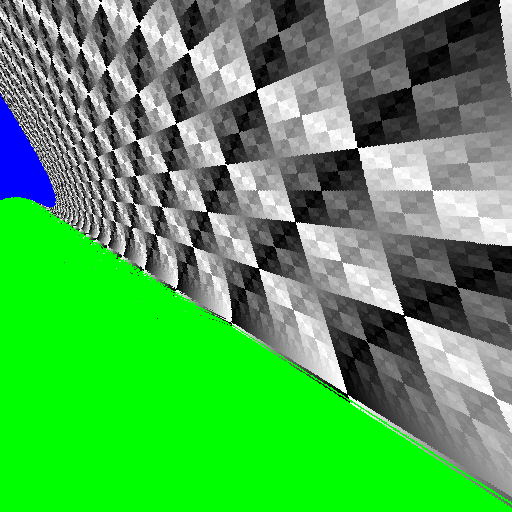
\includegraphics[width=\columnwidth]{sqrt.png}

\section*{Raycasting}

\subsection*{Why raycasting is necessary}

Computer images are (normally, and right now you can pretend that they are always) made of pixels - a 2d lattice of points and associated colors for screen rendering.  If you zoom really far into an image, it gets blurry because the pixels are so sparse.

A lot of rendering today is done by raycasting.  In raycasting, every pixel on the image that is being generated is assigned a vector.  The top left pixel of the image may correspond to a ray that goes in front, above, and to the left of the camera.  Each ray is then tested for intersection with the environment - whether or not it hits something, or where it ends up landing.  Depending on the result (hit/miss, near/far), the pixel corresponding to the ray can be filled in.

\subsection*{Ray tracing}

One technique for raycasting is called ray tracing.  Ray tracing involves mathematically determining the intersections between a line and a surface.  This can be a complicated thing for even simple cases.  To graph $z=e^x$, you would have to solve an intersection between a line and $e^x$.  The Lambert W function exists, but I did not believe (and still do not believe) that I could write a computer program that could automatically do algebra in an efficient manner.

\subsection*{Ray marching}

Another technique for raycasting is called ray marching.  In ray marching, the goal is to gradually move a point along the ray, until the distance between the point and the enviroment surface is 0.  This is where distance functions come in.  If you have a function that tells you the distance to the nearest point on the surface (or at least approximates it), then you know how far along you can move the point before there's a chance that you've moved it too far.

If the distance to the environment surface approaches 0, then my program assumes that the ray hits, and color is a greyscale color which corresponds to the $x$ and $y$ values.  If the distance grows very large, or the program has moved the point along the ray too many times without hitting something, my program assumes that the ray does not hit, and color it blue.  If the distance is undefined (which could happen outside of the domain of the function), then my program colors it green.

\url{https://math.stackexchange.com/questions/2632170/}

\url{https://en.wikipedia.org/wiki/Cube_mapping}

\end{document}
